\section{估计量优良性的判定标准}

虽然总体分布中的参数是确定的, 但是对于同一个参数, 可以有许多不同的点估计. 
在这些估计中, 我们自然地希望挑选一个最“优”的点估计, 因此, 有必要建立评价估计量优劣的标准. 下面介绍几个常用的标准:无偏性、有效性和一致性.

\subsection{无偏性}

\begin{definition}[无偏性]
    \index{无偏性}
    若 $ \hat{\theta}=\hat{\theta}\left(X_{1}, X_{2}, \cdots, X_{n}\right) $ 是参数 $ \theta $ 的估计量, 
    其数学期望 $ E\qty(\hat{\theta}) $ 存在, 且 $ E\qty(\hat{\theta})=\theta $, 则称 $ \hat{\theta} $ \textit{是} $ \theta $ \textit{的无偏估计量}.
\end{definition}

\begin{example}
    已知 $E(X)=\mu, D(X)=\sigma^{2} $ 存在, $ X_{1}, X_{2}, \cdots, X_{n} $ 为来自总体 $ X $ 的样本, 试判定:\label{wpgjllti}
    \begin{enumerate}[label=(\arabic{*})]
        \item $\bar{X} $ 是否为 $ \mu $ 的无偏估计量;
        \item $\displaystyle\frac{1}{n} \sum_{i=1}^{n}\left(X_{i}-\bar{X}\right)^{2} $ 是否为 $ \sigma^{2} $ 的无偏估计量.
    \end{enumerate}
\end{example}
\begin{solution}
    由定义可知, 
    \begin{enumerate}[label=(\arabic{*})]
        \item 因为总体 $ E(X)=\mu, D(X)=\sigma^{2}, X_{1}, X_{2}, \cdots, X_{n} $ 为来自总体 $ X $ 的样本, 则
              $$E\left(X_{i}\right)=\mu, D\left(X_{i}\right)=\sigma^{2}, \quad i=1,2, \cdots, n $$
              所以 $\displaystyle E\qty(\bar{X})=E\qty(\dfrac{1}{n}\sum_{i=1}^{n}X_i)=\dfrac{1}{n}\sum_{i=1}^{n}E(X_i)=\mu$, 
              所以 $\bar{X} $ 为 $ \mu $ 的无偏估计量.
        \item 因为 $\displaystyle D\qty(\bar{X})=D\qty(\dfrac{1}{n}\sum_{i=1}^{n}X_i)=\dfrac{1}{n^2}\sum_{i=1}^{n}D(X_i)=\dfrac{\sigma^2}{n}$, 所以
              $$E\qty(\bar{X}^2)=D\qty(\bar{X})+E^2\qty(\bar{X})=\dfrac{\sigma^2}{n}+\mu^2,~E\qty(X_i^2)=D(X_i)+E^2(X_i)=\sigma^2+\mu^2$$
              \begin{flalign*}
                  E\qty[\dfrac{1}{n}\sum_{i=1}^{n}\qty(X_i-\bar{X})^2] & =E\qty(\dfrac{1}{n}\sum_{i=1}^{n}X_i^2-\bar{X}^2)=\dfrac{1}{n}\sum_{i=1}^{n}E\qty(X_i^2)-E\qty(\bar{X}^2) \\
                                                                       & =\dfrac{1}{n}\sum_{i=1}^{n}\qty(\mu^2+\sigma^2)-\qty(\dfrac{\sigma^2}{n}+\mu^2)=\dfrac{n-1}{n}\sigma^2
              \end{flalign*}
              所以 $\displaystyle\dfrac{1}{n}\sum_{i=1}^{n}\qty(X_i-\bar{X})^2$ 不是 $\sigma^2$ 的无偏估计量.
    \end{enumerate}
\end{solution}

由例题 \ref{wpgjllti} 可以看出, 若在 $ \displaystyle\frac{1}{n} \sum_{i=1}^{n}\left(X_{i}-\bar{X}\right)^{2} $ 前面乘以系数
$ \displaystyle\frac{n}{n-1} $, 就修正成为 $ \sigma^{2} $ 的无偏估计量.
由此也解释了在定义样本方差时, 之所以选择 $\displaystyle S^{2}=\frac{1}{n-1} \sum_{i=1}^{n}\left(X_{i}-\bar{X}\right)^{2}$, 
而不是 $\displaystyle \frac{1}{n} \sum_{i=1}^{n}\left(X_{i}-\bar{X}\right)^{2} $ 形式, 是因为 $ S^{2} $ 是 $ \sigma^{2} $ 的无偏估计量.

\subsection{有效性}

同一个参数可以有多个无偏估计量, 那么选择哪一个为好呢? 设参数 $ \theta $ 有两个无偏估计量 $ \hat{\theta}_{1} $ 和 $ \hat{\theta}_{2}$, 
在样本容量 $ n $ 相同的情况下, 若 $ \hat{\theta}_{1} $ 的观测值都集中在 $ \theta $ 的真值附近, 
而 $\hat{\theta}_{2}$ 的观测值较远离 $\theta$ 的真值, 很显然 $\hat{\theta}_{1}$ 作为 $\theta$ 的估计更合适.
即 $\hat{\theta}_{1}$ 的方差较 $\hat{\theta}_{2}$ 的方差小, 我们认为 $\hat{\theta}_{1}$ 较 $\hat{\theta}_{2}$ 要好, 由此有如下的定义.

\begin{definition}[有效性]
    \index{有效性}
    设 $ \hat{\theta}_{1}=\hat{\theta}_{1}\left(X_{1}, X_{2}, \cdots, X_{n}\right) $ 与 $ \hat{\theta}_{2}=\hat{\theta}_{2}\left(X_{1}, X_{2}, \cdots, X_{n}\right)$
    都是参数 $ \theta $ 的无偏估计量, 若 $ D\left(\hat{\theta}_{1}\right) \leqslant D\left(\hat{\theta}_{2}\right) $, 则称 $ \hat{\theta}_{1} $ \textit{较} $ \hat{\theta}_{2} $ \textit{更有效}.
\end{definition}

% \begin{example}
%     设 $X_{1}, X_{2}, X_{3}, X_{4}$ 是来自均值为 $\theta$ 的指数分布总体的样本, 其中 $\theta$ 未知, 设有估计量
%     \begin{flalign*}
%         T_{1} & =\dfrac{1}{6}\left(X_{1}+X_{2}\right)+\dfrac{1}{3}\left(X_{3}+X_{4}\right), \\
%         T_{2} & =\dfrac{X_{1}+2 X_{2}+3 X_{3}+4 X_{4}}{5},                                  \\
%         T_{3} & =\dfrac{X_{1}+X_{2}+X_{3}+X_{4}}{4} .
%     \end{flalign*}
%     \begin{enumerate}[label=(\arabic{*})]
%         \item 指出 $T_{1}, T_{2}, T_{3}$ 中哪几个是 $\theta$ 的无偏估计量;
%         \item 在上述 $\theta$ 的无偏估计中指出哪一个较为有效.
%     \end{enumerate}
% \end{example}
% \begin{solution}
    
% \end{solution}

\begin{example}
    设总体 $X$ 的概率密度函数为 $f(x,\theta)=\begin{cases}
        \dfrac{3}{\theta^3}x^2,&0\leqslant x\leqslant \theta\\ 0,&\text{其他}
    \end{cases}$其中 $\theta>0$ 为未知参数, $X_1, X_2, \cdots ,X_n~(n>1)$ 是来自总体 $X$ 的样本.
    \begin{enumerate}[label=(\arabic{*})]
        \item 求 $\theta$ 的最大似然估计量 $\hat{\theta}_L$;
        \item 证明: $\hat{\theta}_1=\dfrac{3n+1}{3n}\hat{\theta}_L$ 和 $\hat{\theta}_2=\dfrac{4}{3}\bar{X}$ 均为 $\theta$ 的无偏估计量;
        \item $\hat{\theta}_1$ 和 $\hat{\theta}_2$ 哪一个更有效? 为什么?
    \end{enumerate}
\end{example}
\begin{solution}
    \begin{enumerate}[label=(\arabic{*})]
        \item 由题意得 $\displaystyle L(\theta)=\prod_{i=1}^{n} f(x_i,\theta)=\dfrac{3^n}{\theta^{3n}}\prod_{i=1}^{n}x_i^2~(0\leqslant x_i\leqslant\theta)$, 则 $$
        \ln L(\theta)=n\ln 3-3n\ln\theta+2\sum_{i=1}^{n} \ln x_i~(0\leqslant x_i\leqslant\theta)
        $$
        由 $\displaystyle \pdv{\ln L(\theta)}{\theta}=\dfrac{-3n}{\theta}<0$, 得 $L(\theta)$ 是关于 $\theta$ 单调递减函数, 如图 \ref{zuidasrgjmax} 所示, 
        \begin{figure}[H]
            \centering
            

\tikzset{every picture/.style={line width=0.75pt}} %set default line width to 0.75pt        

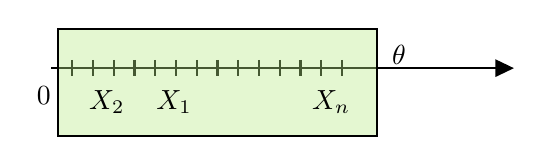
\begin{tikzpicture}[x=0.75pt,y=0.75pt,yscale=-1,xscale=1]
%uncomment if require: \path (0,310); %set diagram left start at 0, and has height of 310

%Straight Lines [id:da02598919413844425] 
\draw    (100,114) -- (250,114) (110,110) -- (110,118)(120,110) -- (120,118)(130,110) -- (130,118)(140,110) -- (140,118)(150,110) -- (150,118)(160,110) -- (160,118)(170,110) -- (170,118)(180,110) -- (180,118)(190,110) -- (190,118)(200,110) -- (200,118)(210,110) -- (210,118)(220,110) -- (220,118)(230,110) -- (230,118)(240,110) -- (240,118) ;
%Straight Lines [id:da8116177486390612] 
\draw    (250,114) -- (319.8,114) ;
\draw [shift={(322.8,114)}, rotate = 180] [fill={rgb, 255:red, 0; green, 0; blue, 0 }  ][line width=0.08]  [draw opacity=0] (8.93,-4.29) -- (0,0) -- (8.93,4.29) -- cycle    ;
%Shape: Rectangle [id:dp8868275986730669] 
\draw  [fill={rgb, 255:red, 184; green, 233; blue, 134 }  ,fill opacity=0.38 ] (103,95) -- (256.8,95) -- (256.8,146.7) -- (103,146.7) -- cycle ;

% Text Node
\draw (100.6,127.35) node   [align=left] {\begin{minipage}[lt]{11.42pt}\setlength\topsep{0pt}
$\displaystyle 0$
\end{minipage}};
% Text Node
\draw (162.2,130.35) node   [align=left] {\begin{minipage}[lt]{17.41pt}\setlength\topsep{0pt}
$\displaystyle X_{1}$
\end{minipage}};
% Text Node
\draw (129.8,130.35) node   [align=left] {\begin{minipage}[lt]{17.41pt}\setlength\topsep{0pt}
$\displaystyle X_{2}$
\end{minipage}};
% Text Node
\draw (237.2,130.35) node   [align=left] {\begin{minipage}[lt]{17.41pt}\setlength\topsep{0pt}
$\displaystyle X_{n}$
\end{minipage}};
% Text Node
\draw (275.8,107.65) node   [align=left] {\begin{minipage}[lt]{17.41pt}\setlength\topsep{0pt}
$\displaystyle \theta $
\end{minipage}};


\end{tikzpicture}
        \caption{}
        \label{zuidasrgjmax}
        \end{figure}
        也就是当 $\theta\geqslant \max\limits_{1\leqslant i\leqslant n}\qty{X_i}$ 时, 
        $\theta$ 的最小值为 $\max\limits_{1\leqslant i\leqslant n}\qty{X_i}$, 因此 $\theta$ 的最大似然估计量为 $\hat{\theta}_L=\max\limits_{1\leqslant i\leqslant n}\qty{X_i}$;
        \item 由 $f(x)$ 的概率密度函数得 
        $$
        F_X=\begin{cases}
            \dfrac{x^3}{\theta^3},&0\leqslant x< \theta\\ 
            0,&x<0\\ 1,&x\geqslant\theta
        \end{cases}
        $$
        并且
        \begin{flalign*}
            EX^2&=\int_{0}^{\theta} \dfrac{3}{\theta^3}x^4 \dd x=\dfrac{3\theta^2}{5}\\ 
            EX&=\int_{0}^{\theta}\dfrac{3}{\theta^3}x^3\dd x=\dfrac{3\theta}{4}
        \end{flalign*}
        所以 $E\hat{\theta}_2=\dfrac{4}{3}\cdot\dfrac{1}{n}\cdot nEX=\dfrac{4}{3}\cdot\dfrac{3\theta}{4}=\theta$, 
        令 $Y=\max\limits_{1\leqslant i\leqslant n}\qty{X_i}$, 则 
        $$F_Y=P\qty{Y\leqslant y}=\qty{\max\limits_{1\leqslant i\leqslant n}\qty{X_i}\leqslant y}=\prod_{i=1}^{n} P\qty{X_i\leqslant y}=P^n\qty{X\leqslant y}=F_X^n(y)=\begin{cases}
            \qty(\dfrac{y^3}{\theta^3})^n,&0\leqslant y< \theta\\ 0,&y<0\\ 1,&y\geqslant\theta
        \end{cases}$$
        那么 $f_Y=F_Y'=\begin{cases}
            \dfrac{3n}{\theta^{3n}}y^{3n-1},& 0< y< \theta\\ 0,&\text{其他}
        \end{cases}$
        因此 
        $$
        E\hat{\theta}_1=\dfrac{3n+1}{3n}E\hat{\theta}_L=\dfrac{3n+1}{3n}EY=(3n+1)\int_{0}^{\theta} \dfrac{y^{3n}}{\theta^{3n}} \dd y=\theta
        $$
        故 $\hat{\theta}_1=\dfrac{3n+1}{3n}\hat{\theta}_L$ 和 $\hat{\theta}_2=\dfrac{4}{3}\bar{X}$ 均为 $\theta$ 的无偏估计量;
        \item 由上述可得
        $$D\hat{\theta}_2=\dfrac{16}{9}D\bar{X}=\dfrac{16}{9}\dfrac{1}{n^2}\cdot nDX=\dfrac{16}{9n}\qty(EX^2-E^2X)=\dfrac{16}{9n}\qty(\dfrac{3\theta^2}{5}-\dfrac{9\theta^2}{16})=\dfrac{\theta^2}{15n}$$
        并且 $$
        EY^2=\int_{0}^{\theta} \dfrac{3n}{\theta^{3n}}y^{3n+1} \dd y=\dfrac{3n}{3n+2}\theta^2
        $$
        故
        $$
        D\hat{\theta}_1=\qty(\dfrac{3n+1}{3n})^2DY=\qty(\dfrac{3n+1}{3n})^2\qty(EY^2-E^2Y)=\qty(\dfrac{3n+1}{3n})^2\cdot\dfrac{3n}{3n+2}\theta^2-\qty(\dfrac{3n+1}{3n})^2\cdot\qty(\dfrac{3n}{3n+1})^2\theta^2=\dfrac{\theta^2}{3n(n+2)}
        $$
        显然, 当 $n>1$ 时, $\dfrac{1}{3n(3n+2)}<\dfrac{1}{15n}$, 因此 $\hat{\theta}_1$ 比 $\hat{\theta}_2$ 更有效.
    \end{enumerate}
\end{solution}

\subsection{一致性}

无偏性和有效性都是在假设样本容量 $n$ 固定的条件下讨论的.
由于估计量是样本的函数,它依赖样本容量 $n$, 自然地, 我们希望一个好的估计量, 当 $n$ 越来越大时, 它与参数的真值几乎一致, 
这就是估计量的一致性或称之为相合性.

\begin{definition}[一致性]
    \index{一致性}
    设 $ \hat{\theta}\left(X_{1}, X_{2}, \cdots, X_{n}\right) $ 为参数 $ \theta $ 的估计量, 当 $ n \to \infty $ 时, $\hat{\theta}\left(X_{1}, X_{2}, \cdots, X_{n}\right) $ 概率收敛于
    $ \theta $, 即对于任意 $ \varepsilon>0 $, 有
    $$\lim _{n \to \infty} P\qty{\qty|\hat{\theta}-\theta|<\varepsilon}=1$$
    则称 $ \hat{\theta} $ \textit{为} $ \theta $ \textit{的相合估计量}.
\end{definition}

\begin{example}
    设总体 $X$ 的概率密度为 $f(x)=\begin{cases}
        2\e ^{-2(x-\theta)}, & x>\theta\\ 0,& x\leqslant \theta
    \end{cases}$ 其中 $\theta>0$ 是未知参数, 从总体 $X$ 中抽取简单随机样本 $X_1, X_2, \cdots ,X_n$, $\hat{\theta}$ 为 $\theta$ 的最大似然估计量. 
    \begin{enumerate}[label=(\arabic{*})]
        \item 求统计量 $\hat{\theta}$ 的分布函数 $F_{\hat{\theta}}(x)$;
        \item 讨论 $\hat{\theta}$ 是否为 $\theta$ 的无偏估计量, 是否为 $\theta$ 的一致估计量;
        \item 求 $\theta$ 的置信水平为 $1-\alpha$ 的最短的置信区间.
    \end{enumerate}
\end{example}
\begin{solution}
    \begin{enumerate}[label=(\arabic{*})]
        \item 似然函数 $\displaystyle L(\theta)=\prod_{i=1}^{n} f(x_i)=2^n\e ^{-2\sum\limits_{i=1}^{n} (x_i-\theta)}$, 则 $\displaystyle \ln L(\theta)=n\ln 2+2n\theta-2\sum_{i=1}^{n} x_i$, 
        由 $\displaystyle \pdv{\ln L(\theta)}{\theta}=2n>0$, 故 $L(\theta)$ 为关于 $\theta$ 的严格单调递增函数, 当 $\theta=\min\limits_{1\leqslant i\leqslant n}\qty{x_i}$ 时, $L(\theta)$ 最大, 
        故 $\theta$ 的最大似然估计量为 $\hat{\theta}=\min\limits_{1\leqslant i\leqslant n}\qty{X_i}$, 总体 $X$ 的分布函数为 $$
        F_X=\begin{cases}
            1-\e ^{-2(x-\theta)},&x>\theta\\ 0, & x\leqslant \theta
        \end{cases}
        $$
        所以, $\hat{\theta}$ 的分布函数为 $$
        F_{\hat{\theta}}(x)=1-[1-F_X(x)]^n=\begin{cases}
            1-\e ^{-2n(x-\theta)}, &x>\theta\\ 0, & x\leqslant \theta.
        \end{cases}
        $$
        \item $\hat{\theta}$ 的密度函数为 $$
        f_{\hat{\theta}}=\begin{cases}
            2n\e ^{-2n(x-\theta)}, & x>\theta\\ 0,& x\leqslant \theta
        \end{cases}
        $$
        那么 
        \begin{flalign*}
            E\hat{\theta}&=\int_{\theta}^{+\infty}2nx \e ^{-2n(x-\theta)}\dd x\xlongequal{x-\theta=t}\int_{0}^{+\infty}2n(\theta+t)\e ^{-2nt}\dd t=\theta+\dfrac{1}{2n}\\ 
            E\hat{\theta}^2& =\int_{\theta}^{+\infty}2nx^2 \e ^{-2n(x-\theta)}\dd x\xlongequal{x-\theta=t}\int_{0}^{+\infty}2n(\theta+t)^2\e ^{-2nt}\dd t=\theta^2+\dfrac{\theta}{n}+\dfrac{1}{2n^2}
        \end{flalign*}
        故 $D \hat{\theta}=E\hat{\theta}^2-E^2\hat{\theta}=\dfrac{1}{4n^2}$, 因为 $E\hat{\theta}\neq\theta$, 所以 $\hat{\theta}$ 不是 $\theta$ 的无偏估计量, 由于 $$
        \lim_{n \to \infty}E\hat{\theta}=\theta,\quad \lim_{n \to \infty}D\hat{\theta}=0
        $$
        所以 $\hat{\theta}$ 是 $\theta$ 的一致估计量;
        \item 令 $Y=\min\limits_{1\leqslant i\leqslant n}\qty{X_i}-\theta$, 则 $Y$ 的密度函数为 $$
        f_Y=\begin{cases}
            2n\e ^{-2ny}, & y>0\\ 0,& y\leqslant 0
        \end{cases}
        $$
        即 $Y\sim E(2n)$, 选择 $a,b~(0\leqslant a<b)$, 使 $b-a$ 最小且满足 $$
        P(a\leqslant Y\leqslant b)=\int_{a}^{b} 2n\e ^{-2ny} \dd y=1-\alpha
        $$
        即 $$
        P\qty(\min\limits_{1\leqslant i\leqslant n}\qty{X_i}-b\leqslant \theta\leqslant \min\limits_{1\leqslant i\leqslant n}\qty{X_i}-a)=\int_{a}^{b} 2n\e ^{-2ny} \dd y=\e ^{-2na}-\e ^{-2nb}=1-\alpha
        $$
        所以 $\theta$ 的置信水平为 $1-\alpha$ 的置信区间为 $$
        \qty[\min\limits_{1\leqslant i\leqslant n}\qty{X_i}-b,\min\limits_{1\leqslant i\leqslant n}\qty{X_i}-a]
        $$
        此时, $\theta$ 的置信水平为 $1-\alpha$ 的置信区间的平均长度 (期望长度) 为 $$
        l=\min\limits_{1\leqslant i\leqslant n}\qty{X_i}-a-\qty(\min\limits_{1\leqslant i\leqslant n}\qty{X_i}-b)=E(b-a)=b-a
        $$
        欲使 $l$ 最短, 即使得 $b-a$ 最小, 于是, 问题转化为如下的极值问题: $$
        \begin{cases}
            \min f(a,b)=b-a\\ 
            s.t. \e ^{-2na}-\e ^{-2nb}=1-\alpha\\ 
            0\leqslant a<b
        \end{cases}
        $$
        \begin{figure}[H]
            \centering
            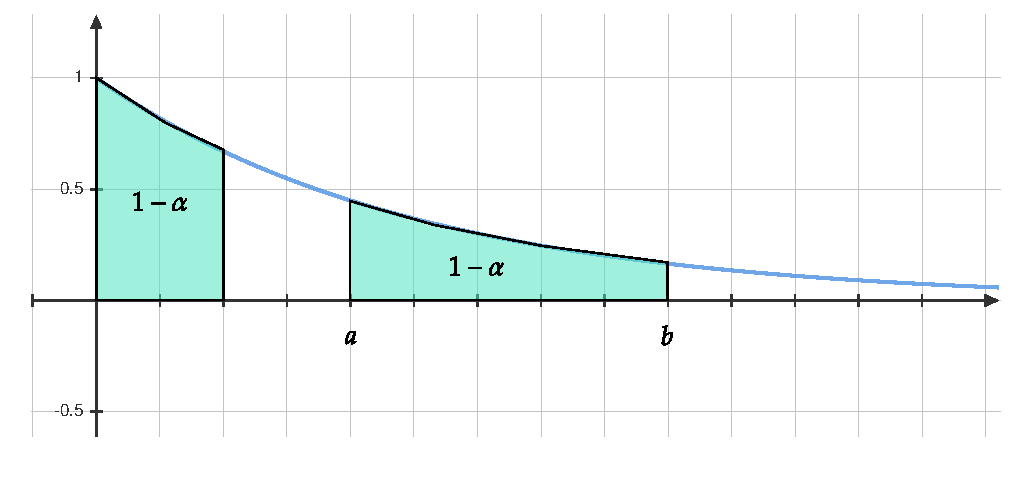
\includegraphics[scale=.6]{figures/diagram-20241129.pdf}
            \caption{}
        \end{figure}
        由于 $2n\e ^{-2ny}~(y\geqslant 0)$ 单调递减, $\displaystyle \int_{a}^{b} 2n\e^{-2ny} \dd y=1-\alpha$ 为常数, 要使得 $b-a$ 最小, 必有 $a=0$, 从而使 
        $$
        \e ^{-2nb}=\alpha\Rightarrow b=-\dfrac{\ln \alpha}{2n}
        $$
        故 $\theta$ 的置信水平为 $1-\alpha$ 的最短的置信区间为 $\qty[X_{(1)}+\dfrac{\ln \alpha}{2n},X_{(1)}]$
        其中 $X_{(1)}=\min\limits_{1\leqslant i\leqslant n}\qty{X_i}.$
        % 因为 $\e ^{-2na}-\e ^{-2nb}=1-\alpha$, 所以 $b=-\dfrac{1}{2n}\ln\qty(\e ^{-2na}+\alpha-1)$, 记 $$
        % g(a)=b-a=-\dfrac{1}{2n}\ln\qty(\e ^{-2na}+\alpha-1)-a
        % $$
        % 因为 $$
        % g'(a)=\dfrac{\e ^{-2na}}{\e ^{-2na}+\alpha-1}-1=\dfrac{1-\alpha}{\e ^{-2na}+\alpha-1}
        % $$
    \end{enumerate}
\end{solution}